\documentclass[]{article}
\usepackage{amsmath}
\usepackage{graphicx}
%opening
%\title{}
%\author{}

\begin{document}



\section{Feature detectors}
	\subsection{Overview}
	\paragraph{Goal of feature/interest point detectors:}
	\begin{itemize}
		\item Detect all 'true' features and no false ones (i.e. high precision, recall)
		\item Well localised points
		\item Robust to noise
		\item Computationally efficient
	\end{itemize}
	\textnormal{The standard approach is to look for regions large gradient changes in x and y directions. If we denote $I(x, y)$ as the intensity at point x,y, then we can calculate the weighted sum of square intensity difference between two images (or a region of an image shifted) with:}
	$$E_{wssd} = \sum_i w(x_i, y_i) [I(x_i+u, y_i+u) - I(x_i, y_i)]^2$$
	\textnormal{where $w(x_i, y_i)$ is the weighting function, in it's simplest case it would be uniform.}
	
	\subsection{Harris Corner Detector}
		\textnormal{Idea: Scan a window over an image and look for significant intensity changes. Use a Taylor series expansion to approximation $I(x_i+u, y_i+v)$: }
		$$I(x_i+u, y_i+v) = I(x_i,y_i) + u\frac{\partial I}{\partial x} (x_i, y_i) + v\frac{\partial I}{\partial y} (x_i, y_i) $$
		\textnormal{This can be represented in matrix form and denoted $\textbf{M}$. In a practical sense the eigenvalues inform us of intensity changes in each direction, such that:}
		\begin{itemize}
			\item if $\lambda_1$ and $\lambda_2$ large then there is a corner  ($ R > 0$)
			\item if $\lambda_1 << | >> \lambda_2$ then there is an edge  ($ R < 0$) 
			\item if both are close to 0, then it is a flat region   ($ R \approx 0$)
		\end{itemize}
		\textnormal{Where $R = Det(M) - ktrace(M)^2$}
		\paragraph{The harris detector is variant to scale, invariant to photometric changes and covariant to geometric (rotational) changes (meaning that the points remain consistent relative to the image).}
		
		\subsubsection{Harris: computational steps}
		\begin{enumerate}
			\item Calculate gradient of image in x and y directions
			\item Calculate $I_x^2$ and $I_y^2$ and $I_xI_y$  (M matrix)
			\item Gaussian blur the image
			\item Calculate R for each point using step 2 results
			\item Choose points with R > 0
			\item Perform non-maximal suppression to localise
		\end{enumerate}
	
	\subsection{Difference of Gaussians (SIFT)}
		\subsubsection{Background: Laplacian of Gaussian (Blob detector)}
		\textnormal{The laplacian of gaussian pics up edge content better than a first order derivative, and traditionally is enhanced to be scale invariant by applying gaussian filters of different sizes to the image first and looking for blobs that are minima/maxima across both space and scale (scale-space). This is a computationally expensive process, and can be estimated using a Difference of Gaussians approach.}
		\subsubsection{Difference of Gaussians approximation}
		$$Lap = \sigma^2(G_xx(x,y,\sigma) + G_yy(x,y,\sigma)) \approx G(x,y,k\sigma) - G(x,y,\sigma)$$
		\paragraph{Steps:}
		\begin{itemize}
			\item Empirically, typical values are $k = \sqrt{2}$ and $\sigma=\frac{1}{\sqrt{2}}$
			\item Apply gaussians with $k\sigma, k^2\sigma, k^3\sigma, ...$ to an image
			\item Downsample the image and repeat (each repeat is an octave)
			\item Subtract two consecutive scales to get the difference
			\item For each min/max found at a scale, compare to neigbouring scales in scale-space and perform non-maximal suppression
			\item (optional) Outlier rejection via thresholding
			\item (Make it orientation invariant) Calculate a histogram of gradients to show the direction of the strongest response in that region
		\end{itemize}
	\newpage		
		\begin{figure}[h!]
			\begin{center}
				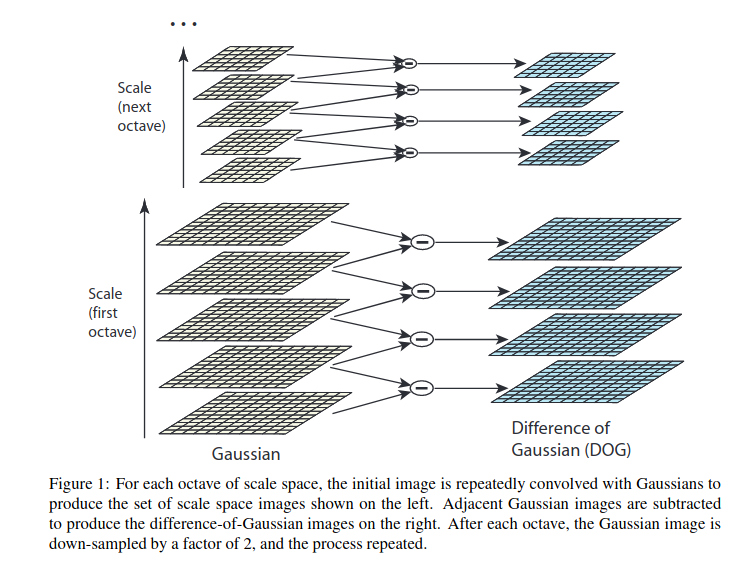
\includegraphics[width=\linewidth]{./images/sift.png}
				\label{fig:sift}
			\end{center}
		\end{figure}
	
		
\section{Feature Extraction}
	\subsection{Overview}
	\textnormal{Feature extraction is the task of extracting the summary statistics of the images and present them in a compact form. It can be done globally (dense) or locally (around interest points). We care about the scope and the content of the features. It has applications in: Image matching, object recognition, object tracking, scene comparison, stereo calibration, robot navigation, image retrieval...}
	\paragraph{Goal of feature extraction:}
	\begin{itemize}
		\item Repeatable, invariant to transform
		\item Discriminates enough
		\item Compact dimensionality
		\item Computationally efficient (corollary to above)
	\end{itemize}
	\subsection{SIFT Descriptor}
	\paragraph{For each interest point:}
	\begin{itemize}
		\item Compute 16x16 patches of magnitude and orientation
		\item Compute HOG for each 4x4 region within the 16x16 (?)
		\item results in a 128D vector
		
	\end{itemize}
	\subsection{Self Similarity Descriptor}
	\paragraph{Looks for repetition in an image. Steps:}
	\begin{itemize}
		\item Take a patch (from interest point, or randomly) and scan it over the image or interest region of the image
		\item Record the correlation at each point
		\item Calculate the log-polar plot and obtain vector representation (can then be used to compare against other images)
		\item Repeat for all patches
	\end{itemize}

	\subsection{LBP and LBP-TOP}
	\paragraph{Good for faces and textures. Steps:}
	\begin{itemize}
		\item Divide image into blocks
		\item For each pixel in each block create an 8 bit score where each bit corresponds to a neighbouring pixels thresholded intensity, 1 if neighbour > subject, 0 otherwise.
		\item Compute the histogram for each block to get the representation for that block
		\item stack histograms together to preserve spatial information.
		\item (repeat for different neighbourhood scales to make it scale invariant)
		\item (LBP-TOP is for video; take 3 orthogonal planes XY, XZ, YZ and compute the same for each)
	\end{itemize}
	
	
\section{Matching features}
	\textnormal{A simple / naive method is to search for matches between groups of interest point regions on two images. A slighly improved version is to do this, but look for the top two matches (for each point) and if the relative similarity is > 0.8 reject the candidate match.}
	
\section{Image Alignment}
	\textnormal{The task of finding parameters of a model (e.g. entries in a matrix) that maps one set of points to another. Tricky in image processing due to noise, outliers, many-to-one object matching.. Basic transforms include scale, shear, rotation, translation, affine, and projective.}
	
	\subsubsection{Example: Panorama stiching} 
	\begin{enumerate}
		\item Compute interest points and match
		\item Compute H (homography matrix) to warp one image to another using matched interest points on edges. use RANSAC method to select the best H:
		\begin{enumerate}
			\item Select set of matched points randomly
			\item Compute the transform for this group
			\item Find the nearest neighbours (the inliers) and count them up
			\item Repeat the process n times
			\item Choose the H that yields the most inliers
		\end{enumerate}
		\item Warp the image using H
	\end{enumerate}
\end{document}